We model a population of sexual organisms evolving in a landscape with two habitat patches connected by dispersal. Two resources are available to the organisms to feed on, and reproductive success is determined by the attack rates of the organisms on the resources. Attack rates on the two resources are determined by an underlying quantitative ecological trait $x$, which is subject to a trade-off so as to favor ecological divergence into two resource specialist strategies. The trait is underlain by a single haploid locus with a continuum of alleles. The ecological trait is also be subject to sexual selection in the form of assortative mating, where females tend to prefer mates with more similar trait values.

\subsection*{Life cycle}

The life cycle of the organisms unfolds in discrete generations. At each generation the population goes through a phase of competition for the limited resources, followed by reproduction, survival and dispersal. Population size is variable and generations overlap.

\paragraph{Competition} Individuals compete for the resources available in their local habitat patch. The competitive ability of an individual depends on its trait value $x$ and determines its reproductive success, or fitness $W_j(x)$ in patch $j$, as follows:

\begin{equation}
    W_j(x) = e_1(x) \, R^*_{1j} + e_2(x) \, R^*_{2j}
\end{equation}

where $e_i(x)$ is the attack rate of individual $k$ on resource $i$ and $R^*_{ij}$ is the equilibrium resource concentration of resource $i$ in patch $j$. The attack rates of individuals on resource $i$ depend on the ecological trait $x$ as follows

\begin{equation}
    e_i(x) = \exp{(-s \, (x \pm 1)^2)}
    \label{eq:attack_rates}
\end{equation}

% Feeding efficiencies depend on the ecological trait
\begin{figure}
    \begin{center}
        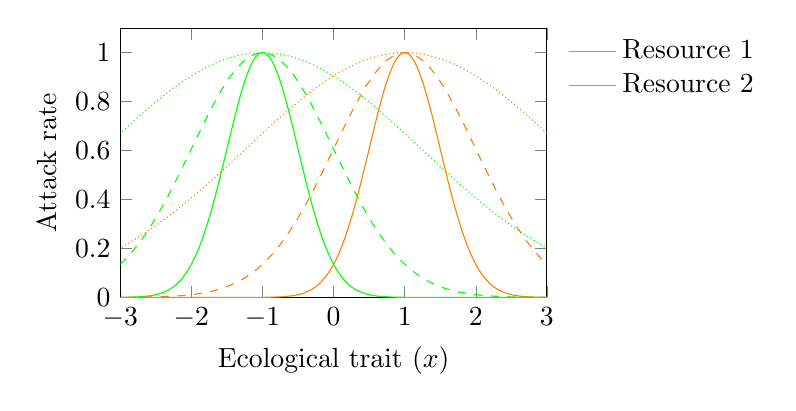
\begin{tikzpicture}
            \begin{axis}[xmin=-3, xmax=3, ymin=0, ymax=1.1, width=7cm, height=5cm, xtick distance=1,ytick distance=0.2, xlabel=Ecological trait ($x$), ylabel=Attack rate, legend entries={Resource 1, Resource 2}, legend style={draw=none, legend pos=outer north east}]
                \addplot[orange, samples=1000] {exp(-2*(x-1)^2)};
                \addplot[green, samples=1000] {exp(-2*(x+1)^2)};
                \addplot[densely dotted, green, samples=100] {exp(-0.1*(x+1)^2)};
                \addplot[dashed, green, samples=100] {exp(-0.5*(x+1)^2)};
                \addplot[densely dotted, orange, samples=100] {exp(-0.1*(x-1)^2)};
                \addplot[dashed, orange, samples=100] {exp(-0.5*(x-1)^2)};
            \end{axis}
            \end{tikzpicture}
        \end{center}
    \label{fig:attack_rates}
    \caption{Attack rate on both resources as a function of the ecological trait. The ecological selection coefficient $s$ determines the strength of the trade-off: dotted lines, $s = 0.1$, dashed lines, $s = 0.5$, solid lines, $s = 2$.}
\end{figure}

where $s$ is the ecological divergent selection coefficient. The respective attack rates on the first and second resource are maximized at values of $x$ of $-1$ and $+1$, which represent specialist strategies. The attack rates are subject to a trade-off, such that organisms cannot have a high payoff on both resources, and whose strength is controlled by $s$. The stronger this ecological trade-off, the more generalist phenotypes, i.e. values of $x$ near zero, suffer reduced attack rates relative to specialist competitors (Fig. \ref{fig:attack_rates}). If $s = 0$ the ecological trait does not affect the attack rates, i.e. there is no selection.\\

The resources flow through the landscape like through a chemostat according to the following dynamics:

\begin{equation}
    \frac{dR_{ij}}{dt} = a \, H_{ij} - \big(b + \sum_{k \in S_j} e_i(x_k) \big) \, R_{ij}
    \label{eq:resource_dynamics}
\end{equation}

where $R_{ij}$ is the concentration of resource $i$ in habitat-patch $j$, $a$ is the absolute rate of resource inflow, $b$ is the relative rate of resource outflow, $H_{ij}$ is a coefficient of symmetry in rates of resource inflow between the two patches, and $e_i(x_k)$ is the attack rate of individual $k$ on resource $i$. The sum of attack rates across the set $S_j$ of individuals living in patch $j$ symbolizes the consumption of the resource by the organisms. The habitat symmetry factor $H_{ij}$ controls the reduction in inflow of resource 2 relative to resource 1 in patch 1, and of resource 1 relative to resource 2 in patch 2, such that the two habitat patches are mirror images of each other with respect to resource inflow,

\begin{equation}
    H = 
    \begin{pmatrix} 
        1 & h \\ 
        h & 1
    \end{pmatrix}
\end{equation}

where $h$ is the habitat symmetry parameter, ranging from 0 to 1. When $h = 1$, the rate of inflow is homogeneous between resources across habitats. On the contrary, when $h = 0$, the landscape is fully heterogeneous in resource inflow, where only resource 1 flows through patch 1 and only resource 2 flows through patch 2. The level of environmental heterogeneity is an important determinant of the mode of speciation that will occur (Rettelbach).\\

We assume that the dynamics of the resources are fast relative to the population dynamics, such that equilibrium resource concentrations are given by solving Equation \ref{eq:resource_dynamics}:

\begin{equation}
    R^*_{ij} = \frac{a \, H_{ij}}{b + \sum_{k \in S_j} e_i(x_k)}
\end{equation}

\paragraph{Reproduction} Females and males encounter each other and mate within patches. We assume a balanced sex ratio. The probability that female $\female$ accepts encountered male $\male$, i.e. the attractiveness of male $\male$ to female $\female$, depends on its ecological trait value and is given by the assortative mating probability function

\begin{equation}
    A(x_{\male}, x_{\female}) = \exp{\big(-\alpha \, (x_{\male} - x_{\female})^2\big)}
    \label{eq:assortative_mating}
\end{equation}

where $\alpha$ is the sexual selection coefficient, scaling the sensitivity of females to deviations in ecological trait values. Females have a* stronger preference for more ecologically similar males as $\alpha$ increases (Fig. \ref{fig:mating_probability}). When $\alpha = 0$, females mate at random.\\ 

\begin{figure}
    \begin{center}
        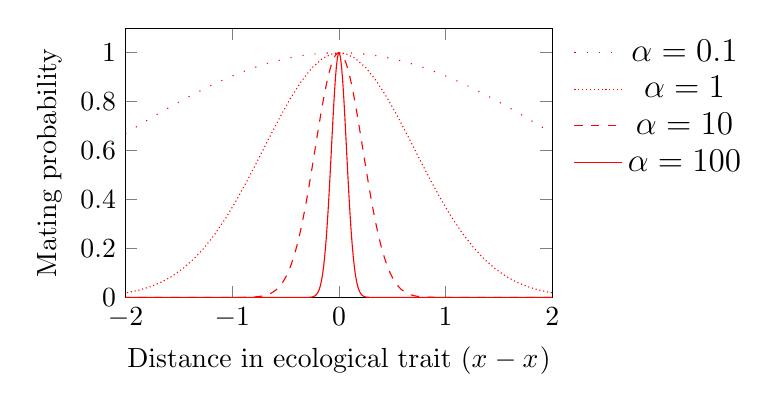
\begin{tikzpicture}
            \begin{axis}[xmin=-2, xmax=2, ymin=0, ymax=1.1, width=7cm, height=5cm, xtick distance=1,ytick distance=0.2, xlabel=Distance in ecological trait ($x_{\male} - x_{\female}$), ylabel=Mating probability, legend entries={$\alpha = 0.1$, $\alpha = 1$, $\alpha = 10$, $\alpha = 100$}, legend style={font=\large, draw=none, legend pos=outer north east}]
                \addplot[loosely dotted, red, samples=100] {exp(-0.1*x^2)};
                \addplot[densely dotted, red, samples=100] {exp(-1*x^2)};
                \addplot[dashed, red, samples=1000] {exp(-10*x^2)};
                \addplot[red, samples=1000] {exp(-100*x^2)};
            \end{axis}
            \end{tikzpicture}
        \end{center}
    \label{fig:mating_probability}
    \caption{Mating probability, or attractiveness, of a male with trait value $x_i$ to a female with trait value $x_j$ for different values of the sexual selection coefficient $\alpha$.}
\end{figure}

The competitive abilities $W_j$ affect the reproductive output of males and females differently. In females, $W_j(x_{\female})$ is the number of offspring that a female can produce. In males, $W_j(x_{\male})$ is analogous the activity of a male on the mating market, and corresponds to the rate of encounter of a male.

\paragraph{Survival} Newborns of the current generation all survive to the next generation and become sexually mature. Generations overlap and adults of the current generation survive with probability $1-d$, where $d$ is the per capita death rate.

\paragraph{Dispersal} At very generation a proportion $m$ of the individuals disperses to the alternative patch.

\subsection*{Adaptive dynamics}

We use adaptive dynamics to analyze the evolutionary outcome of our model under the effects of natural and sexual selection. Adaptive dynamics theory is concerned with the conditions under which an initially rare mutant can spread in a population of resident phenotypes (cite Geritz and Metz). The derivations are simplified by assuming that the resident population is monomorphic with respect to the evolving trait, here $x$. In a model with discrete-time population dynamics, a mutant will spread if its geometric growth rate, or invasion fitness, is higher the growth rate of the resident. Assuming that mutations are rare relative to the population dynamics, that selection is the only force at play (no drift) and that the mutant allele is only slightly deviating from the resident allele in phenotype, a mutant that spreads will invade the population and become the new resident (cite?). If evolution is limited by mutations and occurs through successive allele substitutions, the direction and extent of evolution by selection is described by the selection gradient, which is the change in invasion fitness as the trait value of the mutant changes, given a resident trait value. A positive selection gradient will favor an increase in trait value while a negative selection gradient will favor a decrease. Evolutionary singular strategies are trait values for which the selection gradient is zero, and correspond to either local minima or local maxima in the invasion fitness. A singular strategy that is a local maximum is invasion-proof and is evolutionarily stable strategy under stabilizing selection. A local minimum is a resident trait value that can be invaded by any neighboring mutant and is evolutionarily unstable, that is, it is under disruptive selection and may be a branching point. The evolutionary stability of a singular strategy is given by the curvature of the invasion fitness function at the singular trait value. Not every singular strategy is necessarily attainable through evolution if a population starts off with a different resident trait value. A singular strategy is convergence-stable, or attainable, if it is an attractor for nearby resident trait values. This is the case if the selection gradient pushes for an increase in trait value when slightly below the singular strategy, and for a decrease when slightly above. Otherwise, the singular strategy is an evolutionary repellor, which a population will evolve away from.\\

Assuming small and rare mutational steps and a large and monomorphic population with respect to trait $x$, we can derive a selection gradient, which indicates the direction of evolution. We find evolutionary equilibria as values of $x$ where the selection gradient becomes zero. Speciation is favored if selection leads to those equilibria and favors branching, that is, becomes disruptive once there. Those conditions can be evaluated by studying the attainability and the invasion-proofness of the equilibria, using criteria that can be derived from the selection gradient and the curvature of the fitness function. We are searching for branching points, i.e. equilibrium values of trait $x$ towards which directional selection leads but where the fitness landscape becomes a valley once attained, thus invasible by any neighboring mutant. It is important to note that the shape of the fitness landscape can change as a population evolves, due to frequency-dependent selection. Here, frequency-dependence is present through competition for limited resources.\\

We first describe the dynamics of a mutant population and how they depend on model parameters. We derive the invasion fitness as the geometric growth rate of the mutant. Next, we derive an expression for the selection gradient, the curvature of the fitness function and the attainability of the equilibriq. We show that the location of evolutionary equilibria does not depend on sexual selection, but that sexual selection in the form of assortative mating has a stabilizing effect on the evolution of trait $x$ and may counteract branching. Finally, we explore branching conditions across parameter space by numerically evaluating the previously derived functions, using a \textit{Mathematica} notebook provided in Online Supplements.

\subsection*{Ecological dynamics}

Consider a population of organisms with access to two habitat patches and two resources, just like in our simulation model. The resource dynamics are affected by the consumption by the organisms as in Equation \ref{eq:resource_dynamics}, except that here we assume the population to be monomorphic with respect to the ecological trait $x$. Equation \ref{eq:resource_dynamics} then becomes

\begin{equation}
    \frac{dR_{ij}}{dt} = a \, H_{ij} - (b + e_i(x)\, N_j ) \, R_{ij}
\end{equation}

where $R_{ij}$ is the concentration of resource $i$ in patch $j$ and depends on the number of individuals $N_j$ in patch $j$. The other parameters are described in the main text. The attack rates $e_i(x)$ are given in Equation \ref{eq:attack_rates} and are subject to a trade-off controlled by the ecological selection coefficient $s$ (Fig. \ref{fig:attackrates}).\\

The population dynamics of a rare mutant with ecological trait value $x$ arising in a monomorphic resident population with trait value $\hat{x}$ are

\begin{equation}
    \overrightarrow{N'}_{t+1} = \pmb{\Lambda} \, \overrightarrow{N'}_t
\end{equation}

where $\overrightarrow{N'}_t$ is the vector of mutant population densities across patches, $N'_1$ and $N'_2$, at discrete generation $t$. The transition matrix $\pmb{\Lambda}$ captures the steps of the life cycle of the organism,

\begin{equation}
    \pmb{\Lambda} = \pmb{M} \, \pmb{Q}
\end{equation}

where $\pmb{M}$ is the migration matrix, given by

\begin{equation}
    \pmb{M} =
    \begin{pmatrix}
        1-m & m \\
        m & 1-m 
    \end{pmatrix}
\end{equation}

where $m$ is the migration rate, and $\pmb{Q}$ is the matrix of local per capita growth rates,

\begin{equation}
    \pmb{Q} =
    \begin{pmatrix}
        r_1(x, \hat{x}) & 0 \\
        0 & r_2(x, \hat{x})
    \end{pmatrix}
\end{equation}

The within-patch geometric growth rate captures local competition, reproduction and survival. The local growth rate in patch $j$ is given by

\begin{equation}
    r_j(x, \hat{x}) = 1 - d + \frac{1}{2} \, \Bigg[ W_j(x, \hat{x}) + W_j(\hat{x}, \hat{x}) \, \frac{W_j(x, \hat{x})\,A(x,\hat{x})}{W_j(\hat{x}, \hat{x})\,A(\hat{x},\hat{x})}\Bigg]
    \label{eq:growth_rate}
\end{equation}

where $d$ is the per capita death rate, $W_j(x,\hat{x})$ is the reproductive success of a mutant with trait value $x$ in a resident population with trait $\hat{x}$ in patch $j$, and $A(x, \hat{x})$ is the attractiveness of a male mutant for a resident female.\\

The term $1-d$ represents the survival of adults from one generation to the next. The rest of the equation represents the production of mutant offspring by both males and female, respectively. In females, the reproductive success $W(x, \hat{x})$ directly translates into number of offspring. Males, on the other hand, do not produce offspring directly. Given that the mutant is rare, we assume that mutants only mate with residents, and a mutant male will therefore only contribute to the offspring of a resident female, $W(\hat{x}, \hat{x})$. Males are also subject to sexual selection. Their reproductive output is weighed by their mating success. Male mating success depends on the attractiveness of the male for a resident female, $A(x, \hat{x})$, and on the reproductive success of the male $W(x, \hat{x})$, which in males determines their activity on the mating market. The mating success of the mutant is normalized by the mating success of the resident. Finally, in a haploid system with Mendelian segregation, only half of the offspring of mutants mating with residents will be of mutant phenotype.\\

The reproductive success is the competitive ability of the individual when exploiting the resources,

\begin{equation}
    W_j(x, \hat{x}) = e_1(x) \, R^*_{1j} + e_2(x) \, R^*_{2j}
\end{equation}

where $R^*_{ij}$ is the equilibrium concentration of resource $i$ in patch $j$. Just like in our simulation model we assume fast resource dynamics relative to the population of organisms. We also assume that mutants are rare enough that they have no effect on the equilibrium resource dynamics, such that

\begin{equation}
    R^*_{ij} = \frac{a \, H_{ij}}{b + e_i(\hat{x})\,N_j}
\end{equation}

where the attack rate $e_i(x)$ on resource $i$ is given by

\begin{equation}
    e_i(x) = \exp{(-s\,(x \pm 1)^2)}
\end{equation}

where the optimal attack rate on the first resource is attained for $x = -1$, the optimal attack rate on the second resource is attained for $x = 1$ and $s$ is the divergent ecological selection coefficient, controlling the strength of the trade-off between the two resources (Fig. \ref{fig:attack_rates}).\\

\begin{figure}
    \begin{center}
        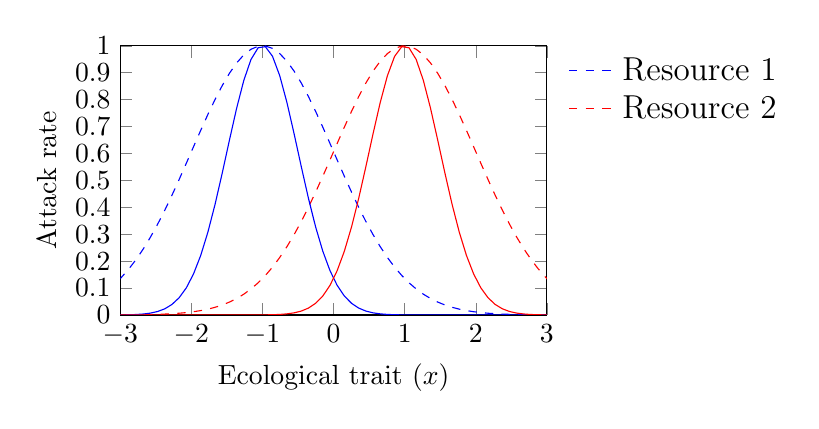
\begin{tikzpicture}
            \begin{axis}[xmin=-3, xmax=3, ymin=0, ymax=1, width=7cm, height=5cm, xtick distance=1,ytick distance=0.1, xlabel=Ecological trait ($x$), ylabel=Attack rate, legend entries={Resource 1, Resource 2}, legend style={font=\large, draw=none, legend pos=outer north east}]
                \addplot[dashed, blue, samples=100] {exp(-0.5*(x+1)^2)};
                \addplot[dashed, red, samples=100] {exp(-0.5*(x-1)^2)};
                \addplot[blue, samples=100] {exp(-2*(x+1)^2)};
                \addplot[red, samples=100] {exp(-2*(x-1)^2)};
            \end{axis}
            \end{tikzpicture}
        \end{center}
    \label{fig:attack_rates}
    \caption{Attack rate on both resources as a function of the ecological trait. The ecological selection coefficient $s$ determines the strength of the trade-off: solid lines, $s = 0.5$, dashed lines, $s = 2$. Here, $e_{max} = 1$.}
\end{figure}

The attractiveness function is the same as the assortative mating function in Equation \ref{eq:assortative_mating}, except that the female mate preference trait $y$ is absent. This is because we are interested in the branching conditions under various degrees of assortative mating and not in the evolution of assortative mating per se. This is also why we do not allow for disassortative mating here. Assortative mating is captured by the sexual selection coefficient $\alpha$ in

\begin{equation}
    A(x, \hat{x}) = \exp{(-\alpha \, (x - \hat{x})^2)}
\end{equation}



Given that $A(\hat{x}, \hat{x}) = 1$, Equation \ref{eq:growth_rate} simplifies to

\begin{equation}
    r_j(x, \hat{x}) = 1 - d + \frac{1}{2} \, W(x, \hat{x}) \, \big(1 + A(x, \hat{x})\big)
\end{equation}

In the following we use the convention $r_j(x, \hat{x}) = r_j$ for readability. The invasion fitness, i.e. the long-term growth rate of the mutant, is the leading eigenvalue of the transition matrix $\pmb{\Lambda}$,

\begin{equation}
    \lambda(x, \hat{x}) = \frac{1}{2} \bigg[(1-m) \, (r_1 + r_2) + \sqrt{(1-m)^2 \, (r_1^2 - 2 \, r_1 \, r_2 + r_2^2) + 4 \, m^2 \, r_1 \, r_2} \bigg]
    \label{eq:invasion_fitness}
\end{equation}

where $\lambda$ is the growth rate of a mutant arising in a resident population at its demographic equilibrium, as defined by trait value $\hat{x}$. The mutant can invade and become the new resident if $\lambda(x, \hat{x}) > 1$, otherwise the mutant goes extinct. Note that $\lambda(\hat{x}, \hat{x}) = 1$. In the following we use the notation $\lambda$ for $\lambda(x, \hat{x})$.

\subsection*{Adaptive dynamics}

\paragraph{Selection gradient} The direction of evolution by selection, assuming small mutational steps and a very large population, is given by the selection gradient,

\begin{equation}
    G(\hat{x}) = \frac{\partial \lambda}{\partial x}\bigg|_{x=\hat{x}}
\end{equation}

which is the derivative of the invasion fitness with respect to the mutant phenotype, evaluated at the resident phenotype. Differentiating Equation \ref{eq:invasion_fitness} is possible but cumbersome, hence we find an expression for the selection gradient using the rule:

\begin{equation}
   \frac{\partial \lambda}{\partial x}\bigg = \frac{1}{\overrightarrow{v}^T\,\overrightarrow{u}} \, \bigg( \overrightarrow{v}^T \, \frac{\partial \pmb{\Lambda}}{\partial x} \, \overrightarrow{u} \bigg)
   \label{eq:deriv_fitness}
\end{equation}

(citation) where $\overrightarrow{v}$ and $\overrightarrow{u}$ are left and right eigenvectors, respectively, of the transition matrix $\pmb{\Lambda}$ associated with the dominant eigenvalue $\lambda$. Possible such eigenvectors are

\begin{equation}
    \overrightarrow{v} = 
    \begin{pmatrix}
        \lambda - (1-m)\,r_2 \\
        m\,r_2 
    \end{pmatrix}
    \label{eq:left_eigenvector}
\end{equation}

and

\begin{equation}
    \overrightarrow{u} = 
    \begin{pmatrix}
        \lambda - (1-m)\,r_2 \\
        m\,r_1
    \end{pmatrix}
\end{equation}

The derivative of the transition matrix $\pmb\Lambda$ with respect to $x$ is

\begin{equation}
    \frac{\partial \pmb{\Lambda}}{\partial x} = \pmb{M} \, \frac{\partial \pmb{Q}}{\partial x}
\end{equation}

where $\partial \pmb{Q} / \partial x$ is a diagonal matrix whose elements are, given for patch $j$,

\begin{equation}
    \frac{\partial r_j}{\partial x} = \frac{1}{2} \, \bigg[\frac{\partial W_j}{\partial x} \, (1 + A(x, \hat{x})) + \frac{\partial A}{\partial x} \, W_j(x, \hat{x})\bigg]
    \label{eq:deriv_local_growth}
\end{equation}

where

\begin{equation}
    \frac{\partial A}{\partial x} = -2 \, \alpha \, (x - \hat{x}) \, A(x, \hat{x})
\end{equation}

Because the selection gradient is evaluated at the resident trait value, where $\partial A / \partial x = 0$ and $A(\hat{x},\hat{x}) = 1$, Equation \ref{eq:deriv_local_growth} reduces to

\begin{equation}
    \frac{\partial r_j}{\partial x}\bigg|_{x=\hat{x}} = \frac{\partial W_j}{\partial x}\bigg|_{x=\hat{x}} 
\end{equation}

Also, given $\lambda(\hat{x}, \hat{x}) = 1$, the eigenvectors $\overrightarrow{v}$ and $\overrightarrow{u}$ evaluated at the resident simplify to

\begin{equation}
    \hat{\overrightarrow{v}} = 
    \begin{pmatrix}
        1 - (1-m)\hat{r}_2\\
        m \, \hat{r}_2
    \end{pmatrix}
    \label{eq:left_eigenvector_resident}
\end{equation}

and

\begin{equation}
    \hat{\overrightarrow{u}} = 
    \begin{pmatrix}
        1 - (1-m)\hat{r}_2\\
        m \, \hat{r}_1
    \end{pmatrix}
    \label{eq:right_eigenvector_resident}
\end{equation}

where 

\begin{equation}
    \hat{r}_j = r_j(\hat{x}, \hat{x}) = 1 - d + W_j(\hat{x}, \hat{x})
    \label{eq:local_growth_resident}
\end{equation}

Substituting Equations \ref{eq:left_eigenvector}--\ref{eq:local_growth_resident} into Equation \ref{eq:deriv_fitness} and simplifying, we get the following expression for the selection gradient:

\begin{equation}
    G(\hat{x}) = \frac{\big[1-m-(2-4\,m+m^2)\,\hat{r}_2+(1-3\,m+2\,m^2)\,\hat{r}^2_2\big]\, \hat{W}_1' + m^2\,\hat{r}_1\,\hat{W}_2'}{(1-\hat{r}_2+m\,\hat{r}_2)^2 + m^2\,\hat{r}_1\,\hat{r}_2}
    \label{eq:fitness_gradient_expression}
\end{equation}

where $\hat{W}_j' = \partial W_j / \partial x |_{x = \hat{x}}$.\\

Hence, the selection gradient does not involve the sexual selection coefficient $\alpha$, and is identical to the selection gradient of an asexual model (show this), whose local growth rate is given by Equation \ref{eq:local_growth_resident}. This means that the equilibrium values of ecological trait $x$, those where the selection gradient is zero, depend on competition, survival and migration, but not on sexual selection. We will now show that sexual selection affects the stability of these equilibria.

\paragraph{Evolutionary stability} The evolutionary stability of an equilibrium trait value $x^*$ depends on the second derivative, or curvature, of the invasion fitness with respect to the mutant phenotype, evaluated at the resident phenotype at evolutionary equilibrium:

\begin{equation}
    \frac{\partial^2 \lambda}{\partial x^2}\bigg|_{x=\hat{x}=x^*}
\end{equation}

If this value is positive, the equilibrium is evolutionarily unstable and the trait value is a fitness minimum, which is a requirement for branching. If this value is negative, the equilibrium is an invasion-proof local maximum, i.e. an evolutionarily stable strategy (ESS) and it cannot branch. It follows from Equation \ref{eq:deriv_fitness} that

\begin{equation}
    \frac{\partial^2 \lambda}{\partial x^2} = \frac{\overrightarrow{v}^T\,\overrightarrow{u}\,\frac{\partial}{\partial x}\,\big(\overrightarrow{v}^T\,\frac{\partial \pmb{\Lambda}}{\partial x}\,\overrightarrow{u}\big) - \frac{\partial}{\partial x} \big( \overrightarrow{v}^T \, \overrightarrow{u} \big) \, \overrightarrow{v}^T \, \frac{\partial \pmb{\Lambda}}{\partial x}\,\overrightarrow{u}}{(\overrightarrow{v}^T\,\overrightarrow{u})^2}
\end{equation}

which, because

\begin{equation}
    \bigg( \overrightarrow{v}^T\,\frac{
    \partial \pmb \Lambda}{\partial x}\,\overrightarrow{u} \bigg)_* = G(x^*) = 0
\end{equation}

simplifies, at equilibrium $x^*$, to

\begin{equation}
    \frac{\partial^2 \lambda}{\partial x^2}\bigg|_* = \Bigg[ \frac{1}{\overrightarrow{v}^T\,\overrightarrow{u}}\,\frac{\partial}{\partial x}\,\bigg(\overrightarrow{v}^T\,\frac{\partial \pmb{\Lambda}}{\partial x}\,\overrightarrow{u}\bigg) \Bigg]_*
    \label{eq:fitness_curvature_equilibrium}
\end{equation}

where

\begin{equation}
    \frac{\partial}{\partial x} \, \bigg(\overrightarrow{v}^T \, \frac{\partial \pmb{\Lambda}}{\partial x} \, \overrightarrow{u}\bigg) = \frac{\partial \overrightarrow{v}^T}{\partial x}\,\frac{\partial \pmb{\Lambda}}{\partial x}\,\overrightarrow{u} + \overrightarrow{v}^T\,\frac{\partial^2 \pmb{\Lambda}}{\partial x^2}\,\overrightarrow{u} + \overrightarrow{v}^T\,\frac{\partial \pmb{\Lambda}}{\partial x}\,\frac{\partial \overrightarrow{u}}{\partial x}
    \label{eq:deriv_num_gradient_unevaluated}
\end{equation}

where the derivatives of the left and right eigenvectors are given by

\begin{equation}
    \frac{\partial \overrightarrow{v}}{\partial x} = 
    \begin{pmatrix}
        \nicefrac{\partial \lambda}{\partial x} - (1-m)\,\nicefrac{\partial r_2}{\partial x}\\
        m\,\nicefrac{\partial r_2}{\partial x}
    \end{pmatrix}
\end{equation}

and

\begin{equation}
    \frac{\partial \overrightarrow{u}}{\partial x} = 
    \begin{pmatrix}
        \nicefrac{\partial \lambda}{\partial x} - (1-m)\,\nicefrac{\partial r_2}{\partial x}\\
        m\,\nicefrac{\partial r_1}{\partial x}
    \end{pmatrix}
\end{equation}

which, because $\partial r_j / \partial x = \partial W_j / \partial x$ at the resident $\hat x$ and $\partial \lambda / \partial x = 0$ at the equilibrium $x^*$, respectively evaluate to

\begin{equation}
    \frac{\partial \overrightarrow{v}}{\partial x}\bigg|_{x=\hat x=x^*} = 
    \begin{pmatrix}
        (m-1)\,\nicefrac{\partial W_2}{\partial x}\\
        m\,\nicefrac{\partial W_2}{\partial x}
    \end{pmatrix}
    _{x=\hat x=x^*}
\end{equation}

and

\begin{equation}
    \frac{\partial \overrightarrow{u}}{\partial x}\bigg|_{x=\hat x=x^*} = 
    \begin{pmatrix}
        (m-1)\,\nicefrac{\partial W_2}{\partial x}\\
        m\,\nicefrac{\partial W_1}{\partial x}
    \end{pmatrix}
    _{x=\hat x=x^*}
    \label{eq:right_eigenvector_equilibrium}
\end{equation}

and where the second derivative of the transition matrix is given by 

\begin{equation}
    \frac{\partial^2 \pmb{\Lambda}}{\partial x^2} = \pmb{M} \, \frac{\partial^2 \pmb{Q}}{\partial x^2}
    \label{eq:second_derivative_transition}
\end{equation}

where $\partial^2 \pmb{Q} / \partial x^2$ is a diagonal matrix whose elements for each patch $j$ are given by differentiating Equation \ref{eq:deriv_local_growth}:

\begin{equation}
    \frac{\partial^2 r_j}{\partial x^2} = \frac{1}{2} \bigg[\frac{\partial^2 W_j}{\partial x^2}\,\big(1+A(x,\hat{x})\big) + 2\,\frac{\partial W_j}{\partial x}\,\frac{\partial A}{\partial x} + \frac{\partial^2 A}{\partial x^2}\,W_j(x,\hat{x})\bigg]
\end{equation}

where

\begin{equation}
    \frac{\partial^2 A}{\partial x^2} = -2\,\alpha\,\big( A(x,\hat{x}) + (x-\hat{x})\,\nicefrac{\partial A}{\partial x} \big)
\end{equation}

which, at equilibrium $x=\hat{x}=x^*$ becomes

\begin{equation}
    \frac{\partial^2 A}{\partial x^2}\bigg|_{x=\hat{x}=x^*} = -2\,\alpha
\end{equation}

The second derivatives of the local growth rates therefore simplify to

\begin{equation}
    \frac{\partial^2 r_j}{\partial x^2}\bigg|_{x=\hat{x}=x^*}= \frac{\partial^2 W_j}{\partial x^2}\bigg|_{x=\hat{x}=x^*} - \alpha \, W_j(x^*,x^*)
    \label{eq:second_derivative_local_growth_equilibrium}
\end{equation}

By substituting Equations \ref{eq:left_eigenvector_resident}, \ref{eq:right_eigenvector_resident} and \ref{eq:deriv_num_gradient_unevaluated}--\ref{eq:second_derivative_local_growth_equilibrium} into Equation \ref{eq:fitness_curvature_equilibrium} and simplifying, we obtain an expression for the curvature of the fitness function at equilibrium:

\begin{equation}
    \begin{split}
        \frac{\partial^2 \lambda}{\partial x^2}\bigg|_{x=\hat x=x^*}=&\frac{1}{1 + m^2\,r^*_1\,r^*_2 + (m - 1)\,\big(2 + (m - 1)\,r^*_2^2\big)} \times \\
        &\Bigg[m^2\, r^*_ 1\, W''^*_2 + 2\, (2\, m - 1)\, \big(1 + (m - 1)\, r^*_ 2\big)\, W'^*_1 \, W'^*_2 +\\
        &\big(1 + (m - 1) \, r^*_ 2\big)\, \big(1 - m + (2 m - 1) \,r^*_ 2\big)\, W''^*_1 -\\
        &\alpha \times \Big(m^2\, r^*_ 1\, W^*_2 - \\
        & \big(m - 1 + (2 - 4\,m + m^2)\, r^*_ 2 - (1 - 3\,m + 2\,m^2)\,r^*_ 2^2\big)\,W^*_1 \Big)\Bigg]
    \end{split}
    \label{eq:fitness_curvature_equilibrium_expression}
\end{equation}

where $W_j^* = W_j(x^*, x^*)$, $W_j''^* = \partial^2 W_j / \partial x^2 |_{x=\hat{x}=x^*}$ and $r_j^* = r_j(x^*, x^*)$.\\

We used this expression to assess the stability of evolutionary equilibria. We will now show that the fitness curve gets more concave at equilibrium as the sexual selection coefficient $\alpha$ increases, i.e. that assortative mating has a stabilizing effect on evolutionary equilibria and may prevent branching. For this, assume that the local per capita growth rate $r_j$ depends on two traits, $x$, which affects competitive ability, and $y$, which affects attractiveness. Those two traits are eventually the same, but we split them to study the effect of the ecological trait on ecological and sexual selection separately. We first show that $x$ and $y$ have independent effects on the curvature of the fitness function at equilibrium, that is,

\begin{equation}
    \frac{\partial^2 \lambda}{\partial x \partial y}\bigg|_* = 0
\end{equation}

where $*$ symbolizes $x=\hat x=x^*$, $y=\hat y=y^*$. The cross-derivative of the fitness function with respect to $x$ and $y$ is

\begin{equation}
    \frac{\partial^2 \lambda}{\partial x \partial y} = \frac{\partial}{\partial y}\,\Bigg[\frac{1}{\overrightarrow{v}^T\,\overrightarrow{u}}\,\bigg( \overrightarrow{v}^T\,\frac{\partial \Lambda}{\partial x}\,\overrightarrow{u} \bigg)\Bigg]
\end{equation}

which is equivalent to

\begin{equation}
    \frac{\partial^2 \lambda}{\partial x \partial y} = \frac{\frac{\partial}{\partial y}\Big(\overrightarrow{v}^T\,\frac{\partial \pmb \Lambda}{\partial x}\,\overrightarrow{u}\Big)\,\overrightarrow{v}^T\,\overrightarrow{u}-\frac{\partial}{\partial y}\,\Big(\overrightarrow{v}^T\,\overrightarrow{u}\Big)\,\Big(\overrightarrow{v}^T\,\frac{\partial \pmb \Lambda}{\partial x}\,\overrightarrow{u}\Big)}{(\overrightarrow{v}^T\,\overrightarrow{u})^2}
\end{equation}

in which

\begin{equation}
    \bigg(\overrightarrow{v}^T\,\frac{\partial \pmb \Lambda}{\partial x}\,\overrightarrow{u}\bigg)_* = 0
\end{equation}

as it corresponds to the fitness gradient, and

\begin{equation}
    \frac{\partial}{\partial y}\,\bigg(\overrightarrow{v}^T\,\frac{\partial \pmb \Lambda}{\partial x}\,\overrightarrow{u}\bigg) = \frac{\partial \overrightarrow{v}^T}{\partial y}\,\frac{\partial \pmb \Lambda}{\partial x}\,\overrightarrow{u}+\overrightarrow{v}^T\,\frac{\partial^2 \pmb \Lambda}{\partial x \partial y}\,\overrightarrow{u}+\overrightarrow{v}^T\,\frac{\partial \pmb \Lambda}{\partial x}\,\frac{\partial \overrightarrow{u}}{\partial y}   
    \label{eq:deriv_lambda_x_y}
\end{equation}

where the derivatives of the left and right eigenvectors with respect to $y$ are, respectively,

\begin{equation}
    \frac{\partial \overrightarrow{v}}{\partial y} =
    \begin{pmatrix}
        \nicefrac{\partial \lambda}{\partial y} - (1-m)\,\nicefrac{\partial r_2}{\partial y}\\
        m \,\nicefrac{\partial r_2}{\partial y}
    \end{pmatrix}
\end{equation}

and

\begin{equation}
    \frac{\partial \overrightarrow{u}}{\partial y} =
    \begin{pmatrix}
        \nicefrac{\partial \lambda}{\partial y} - (1-m)\,\nicefrac{\partial r_2}{\partial y}\\
        m \,\nicefrac{\partial r_1}{\partial y}
    \end{pmatrix}
\end{equation}

where $\partial \lambda / \partial y = 0$ at equilibrium $x^*$, $y^*$, and

\begin{equation}
    \frac{\partial r_j}{\partial y}\bigg|_* = \frac{1}{2} \, \frac{\partial A}{\partial y}\bigg|_*\,W_j(x^*,x^*)
\end{equation}

where $\partial A / \partial y = 0$ at equilibrium $y^*$. Therefore, both $\partial \overrightarrow{v} / \partial y$ and $\partial \overrightarrow{u} / \partial y$ are vectors of zeros at equilibrium. The cross-derivative of the transition matrix is

\begin{equation}
    \frac{\partial^2 \pmb \Lambda}{\partial x \partial y} = \pmb M \, \frac{\partial}{\partial y}\,\frac{\partial \pmb Q}{\partial x}
\end{equation}

where 

\begin{equation}
    \frac{\partial \pmb Q}{\partial x} = \frac{1}{2}\,\big(1+A(y,\hat y)\big)\,\pmb M \frac{\partial \pmb W}{\partial x}
\end{equation}

where $\pmb W$ is independent of trait $y$ and so

\begin{equation}
    \frac{\partial}{\partial y}\,\frac{\partial \pmb Q}{\partial x} = \frac{1}{2}\,\frac{\partial A}{\partial y}\,\pmb M\,\frac{\partial \pmb W}{\partial x}
\end{equation}

which also reduces to zero at equilibrium and therefore, 

\begin{equation}
    \frac{\partial^2 \lambda}{\partial x \partial y}\bigg|_* = 0
\end{equation}

therefore competition and mate choice  have independent effects on the stability of equilibria. The effect of mate choice on the stability of an equilibrium is given by

\begin{equation}
    \frac{\partial^2 \lambda}{\partial y^2}\bigg|_*
\end{equation}

If this expression is negative, sexual selection is stabilizing the evolutionary dynamics of the ecological trait and may prevent branching. The curvature of the fitness function with respect to $y$ is given by

\begin{equation}
    \frac{\partial^2 \lambda}{\partial y^2} = \frac{1}{\overrightarrow{v}^T\,\overrightarrow{u}}\,\bigg(\overrightarrow{v}^T\frac{\partial \pmb \Lambda}{\partial y}\,\overrightarrow{u}\bigg)
\end{equation}

where 

\begin{equation}
    \frac{\partial \pmb \Lambda}{\partial y} = \pmb M \frac{\partial \pmb Q}{\partial y}
\end{equation}

where

\begin{equation}
    \frac{\partial \pmb Q}{\partial y} = \frac{1}{2}\,\frac{\partial A}{\partial y}\,W(x,\hat x)
\end{equation}

therefore reducing to

\begin{equation}
    \frac{\partial^2 \lambda}{\partial y^2} = \frac{1}{2}\,\frac{\partial}{\partial y}\,\bigg(\frac{\partial A}{\partial y}\, \frac{\overrightarrow{v}^T\,\pmb W\,\overrightarrow{u}}{\overrightarrow{v}^T\,\overrightarrow{u}}\bigg)
\end{equation}

which is equivalent to

\begin{equation}
    \frac{\partial^2 \lambda}{\partial y^2} = \frac{1}{2}\,\frac{\frac{\partial}{\partial y}\,\Big(\frac{\partial A}{\partial y}\,\overrightarrow{v}^T\,\pmb W\,\overrightarrow{u}\Big)\,\overrightarrow{v}^T\,\overrightarrow{u}-\frac{\partial}{\partial y}\Big(\overrightarrow{v}^T\,\overrightarrow{u}\Big)\frac{\partial A}{\partial y}\,\Big(\overrightarrow{v}^T\,\pmb W\,\overrightarrow{u}\Big)}{(\overrightarrow{v}^T\,\overrightarrow{u})^2}
\end{equation}

where $\partial A / \partial y = 0$ at equilibrium and which therefore simplifies to

\begin{equation}
    \frac{\partial^2 \lambda}{\partial y^2}\bigg|_* = \frac{1}{2}\,\Bigg(\frac{1}{\overrightarrow{v}^T\,\overrightarrow{u}}\,\frac{\partial}{\partial y}\,\bigg[\frac{\partial^2 A}{\partial y^2}\,\Big(\overrightarrow{v}^T\,\pmb W\,\overrightarrow{u}\Big)+\frac{\partial A}{\partial y}\,\frac{\partial \big(\overrightarrow{v}^T\,\pmb W\,\overrightarrow{u}\big)}{\partial y}\bigg]\Bigg)_*
\end{equation}

which further simplifies to

\begin{equation}
    \frac{\partial^2 \lambda}{\partial y^2}\bigg|_* = \frac{1}{2}\,\Bigg(\frac{\overrightarrow{v}^T\,\pmb W\,\overrightarrow{u}}{\overrightarrow{v}^T\,\overrightarrow{u}}\,\frac{\partial^2 A}{\partial y}\Bigg)_* = -\alpha \, \Bigg(\frac{\overrightarrow{v}^T\,\pmb W\,\overrightarrow{u}}{\overrightarrow{v}^T\,\overrightarrow{u}}\Bigg)_*
    \label{eq:curvature_final}
\end{equation}

where 

\begin{equation}
    \overrightarrow{v}^*^T\,\overrightarrow{u}^* = \big(1-(1-m)\,r^*_2\big)^2 + m^2\,r^*_1\,r^*_2 > 0
\end{equation}

assuming that the per capita growth rates $r^*_j$ have the same sign, and whose sign is therefore given by the numerator,

\begin{equation}
    \overrightarrow{v}^*^T\,\pmb W^*\,\overrightarrow{u}^* = \big(1-(1-m)\,r^*_2\big)^2\,W^*_1 + m^2\,r^*_1\,r^*_2\,W^*_2
\end{equation}

which is also positive. Therefore, the curvature of the fitness function $\partial^2 \lambda / \partial y^2$ at equilibrium depends negatively on the sexual selection coefficient $\alpha$, i.e. assortative mating brings stabilizing sexual selection into the evolutionary dynamics.

\paragraph{Convergence stability} Last, attainability, or convergence stability, of an equilibrium $x^*$ is guaranteed if the selection gradient favors increasing $x$ when $x < x^*$ but decreasing $x$ when $x > x^*$, that is

\begin{equation}
    \frac{\partial G}{\partial \hat{x}}\bigg|_{\hat{x}=x^*} < 0
\end{equation}

where 

\begin{equation}
    \frac{\partial G}{\partial \hat{x}} = \frac{\partial}{\partial \hat{x}} \Bigg[ \frac{1}{\hat{\overrightarrow{v}}^T\,\hat{\overrightarrow{u}}} \bigg( \hat{\overrightarrow{v}}^T\,\frac{\partial \pmb{\Lambda}}{\partial x}\bigg|_{x=\hat{x}}\,\hat{\overrightarrow{u}} \bigg) \Bigg]
\end{equation}

which is equivalent to

\begin{equation}
    \frac{\partial G}{\partial \hat{x}} = \frac{\frac{\partial}{\partial \hat{x}} \big( \hat{\overrightarrow{v}}^T\,\frac{\partial \pmb{\Lambda}}{\partial x}\big|_{x=\hat{x}}\,\hat{\overrightarrow{u}} \big)\,\hat{\overrightarrow{v}}^T\,\hat{\overrightarrow{u}} - \big( \hat{\overrightarrow{v}}^T\,\frac{\partial \pmb{\Lambda}}{\partial x}\big|_{x=\hat{x}}\,\hat{\overrightarrow{u}} \big)\,\frac{\partial}{\partial \hat{x}} \big(\hat{\overrightarrow{v}}^T\,\hat{\overrightarrow{u}}\big)}{(\hat{\overrightarrow{v}}^T\,\hat{\overrightarrow{u}})^2}
    \label{eq:deriv_gradient}
\end{equation}

which, because

\begin{equation}
    \bigg( \overrightarrow{v}^T\,\frac{\partial \pmb \Lambda}{\partial x}\,\overrightarrow{u} \bigg)_* = G(x^*) = 0
    \label{eq:gradient_is_zero_at_equilibrium}
\end{equation}

simplifies, at equilibrium $x^*$, to

\begin{equation}
    \frac{\partial G}{\partial \hat x}\bigg|_* = \Bigg[ \frac{1}{\hat{\overrightarrow{v}}\,\hat{\overrightarrow{u}}} \, \frac{\partial}{\partial \hat x}\,\bigg(\hat{\overrightarrow{v}}^T\,\frac{\partial \pmb \Lambda}{\partial x}\bigg|_{x=\hat x}\,\hat{\overrightarrow{u}}\bigg)\Bigg]_*
    \label{eq:deriv_gradient_equilibrium}
\end{equation}

where

\begin{equation}
    \frac{\partial}{\partial \hat{x}} \bigg( \hat{\overrightarrow{v}}^T\,\frac{\partial \pmb{\Lambda}}{\partial x}\bigg|_{x=\hat{x}}\,\hat{\overrightarrow{u}} \bigg) = \frac{\partial \hat{\overrightarrow{v}}^T}{\partial \hat{x}}\,\frac{\partial \pmb{\Lambda}}{\partial x}\bigg|_{x=\hat{x}}\,\hat{\overrightarrow{u}} + \hat{\overrightarrow{v}}^T\,\frac{\partial}{\partial \hat{x}} \bigg(\frac{\partial \pmb{\Lambda}}{\partial x}\bigg|_{x=\hat{x}}\bigg)\,\hat{\overrightarrow{u}} + \hat{\overrightarrow{v}}^T\,\frac{\partial \pmb{\Lambda}}{\partial x}\bigg|_{x=\hat{x}}\,\frac{\partial \hat{\overrightarrow{u}}}{\partial \hat{x}}
\end{equation}

where $\partial \pmb \Lambda / \partial x = \pmb M \, \partial \pmb W / \partial x$ at the resident $\hat x$ and therefore

\begin{equation}
    \frac{\partial}{\partial \hat x}\,\bigg(\frac{\partial \pmb \Lambda}{\partial x}\bigg|_{x=\hat x}\bigg) = \pmb M \, \frac{\partial}{\partial \hat x}\,\bigg(\frac{\partial \pmb W}{\partial x}\bigg|_{x=\hat x}\bigg)
\end{equation}

and where the change in left and right eigenvectors evaluated at the resident, as the resident changes, are

\begin{equation}
    \frac{\partial \hat{\overrightarrow{v}} }{\partial \hat x} = 
    \begin{pmatrix}
        (m-1)\,\nicefrac{\partial \hat r_2}{\partial \hat x}\\
        m\,\nicefrac{\partial \hat r_2}{\partial \hat x}
    \end{pmatrix}
    \label{eq:deriv_left_eigenvector_resident}
\end{equation}

and

\begin{equation}
    \frac{\partial \hat{\overrightarrow{u}} }{\partial \hat x} = 
    \begin{pmatrix}
        (m-1)\,\nicefrac{\partial \hat r_2}{\partial \hat x}\\
        m\,\nicefrac{\partial \hat r_1}{\partial \hat x}
    \end{pmatrix}
    \label{eq:deriv_right_eigenvector_resident}
\end{equation}

where $\hat r_j(\hat x) = r_j(\hat x, \hat x)$ is the local growth rate of the resident. The local growth rate is a function of the equilibrium resource concentrations $R^*_{ij}(\hat x)$, which are themselves functions of the equilibrium population densities $N^*_j(\hat x)$ in each patch. The equilibrium population densities depend in return on the equilibrium resource concentrations $R^*_{ij}(\hat x)$ and are found, for a given resident trait value $\hat x$, by solving the resident ecological dynamics:

\begin{equation}
    \pmb \Lambda(\hat x)
    \begin{pmatrix}
        N^*_1(\hat x)\\
        N^*_2(\hat x)
    \end{pmatrix}
    =
    \begin{pmatrix}
        N^*_1(\hat x)\\
        N^*_2(\hat x) 
    \end{pmatrix}
\end{equation}

which are third-degree rational equations in $N^*_1$ and $N^*_2$, which we could not solve analytically. Therefore, we could not obtain explicit expressions for the derivatives of $N^*_1$ and $N^*_2$ with respect to the resident trait value $\hat x$, which are needed to compute the derivatives of the local growth rates $\hat r_j(\hat x)$ in the derivatives of the eigenvectors in Equations \ref{eq:deriv_left_eigenvector_resident} and \ref{eq:deriv_right_eigenvector_resident}, respectively. Instead, we used differences in selection gradient close to the singular points to calculate the convergence stability criterion.

\subsection*{Numerical procedures}

We numerically explored phenotype space for evolutionary equilibria $x^*$ by solving the root of the fitness gradient given in Equation \ref{eq:fitness_gradient_expression} across a range of parameter combinations. For each equilibrium we assessed its convergence and evolutionary stability by evaluating the fitness curvature (Equation \ref{eq:fitness_curvature_equilibrium_expression}) and the change in the direction of the gradient, respectively. Convergent stable but evolutionarily unstable equilibria were classified as branching points. The procedure is shown in the accompanying \textit{Mathematica} notebook. The results of our exploration of parameter space are shown in Figure \ref{fig:adaptive_dynamics}.




